\documentclass[]{article}
\usepackage{lmodern}
\usepackage{amssymb,amsmath}
\usepackage{ifxetex,ifluatex}
\usepackage{fixltx2e} % provides \textsubscript
\ifnum 0\ifxetex 1\fi\ifluatex 1\fi=0 % if pdftex
  \usepackage[T1]{fontenc}
  \usepackage[utf8]{inputenc}
\else % if luatex or xelatex
  \ifxetex
    \usepackage{mathspec}
  \else
    \usepackage{fontspec}
  \fi
  \defaultfontfeatures{Ligatures=TeX,Scale=MatchLowercase}
\fi
% use upquote if available, for straight quotes in verbatim environments
\IfFileExists{upquote.sty}{\usepackage{upquote}}{}
% use microtype if available
\IfFileExists{microtype.sty}{%
\usepackage{microtype}
\UseMicrotypeSet[protrusion]{basicmath} % disable protrusion for tt fonts
}{}
\usepackage[margin=1in]{geometry}
\usepackage{hyperref}
\hypersetup{unicode=true,
            pdftitle={Capstone Project Statistical Report},
            pdfauthor={Tony Tushar Jr},
            pdfborder={0 0 0},
            breaklinks=true}
\urlstyle{same}  % don't use monospace font for urls
\usepackage{color}
\usepackage{fancyvrb}
\newcommand{\VerbBar}{|}
\newcommand{\VERB}{\Verb[commandchars=\\\{\}]}
\DefineVerbatimEnvironment{Highlighting}{Verbatim}{commandchars=\\\{\}}
% Add ',fontsize=\small' for more characters per line
\usepackage{framed}
\definecolor{shadecolor}{RGB}{248,248,248}
\newenvironment{Shaded}{\begin{snugshade}}{\end{snugshade}}
\newcommand{\KeywordTok}[1]{\textcolor[rgb]{0.13,0.29,0.53}{\textbf{#1}}}
\newcommand{\DataTypeTok}[1]{\textcolor[rgb]{0.13,0.29,0.53}{#1}}
\newcommand{\DecValTok}[1]{\textcolor[rgb]{0.00,0.00,0.81}{#1}}
\newcommand{\BaseNTok}[1]{\textcolor[rgb]{0.00,0.00,0.81}{#1}}
\newcommand{\FloatTok}[1]{\textcolor[rgb]{0.00,0.00,0.81}{#1}}
\newcommand{\ConstantTok}[1]{\textcolor[rgb]{0.00,0.00,0.00}{#1}}
\newcommand{\CharTok}[1]{\textcolor[rgb]{0.31,0.60,0.02}{#1}}
\newcommand{\SpecialCharTok}[1]{\textcolor[rgb]{0.00,0.00,0.00}{#1}}
\newcommand{\StringTok}[1]{\textcolor[rgb]{0.31,0.60,0.02}{#1}}
\newcommand{\VerbatimStringTok}[1]{\textcolor[rgb]{0.31,0.60,0.02}{#1}}
\newcommand{\SpecialStringTok}[1]{\textcolor[rgb]{0.31,0.60,0.02}{#1}}
\newcommand{\ImportTok}[1]{#1}
\newcommand{\CommentTok}[1]{\textcolor[rgb]{0.56,0.35,0.01}{\textit{#1}}}
\newcommand{\DocumentationTok}[1]{\textcolor[rgb]{0.56,0.35,0.01}{\textbf{\textit{#1}}}}
\newcommand{\AnnotationTok}[1]{\textcolor[rgb]{0.56,0.35,0.01}{\textbf{\textit{#1}}}}
\newcommand{\CommentVarTok}[1]{\textcolor[rgb]{0.56,0.35,0.01}{\textbf{\textit{#1}}}}
\newcommand{\OtherTok}[1]{\textcolor[rgb]{0.56,0.35,0.01}{#1}}
\newcommand{\FunctionTok}[1]{\textcolor[rgb]{0.00,0.00,0.00}{#1}}
\newcommand{\VariableTok}[1]{\textcolor[rgb]{0.00,0.00,0.00}{#1}}
\newcommand{\ControlFlowTok}[1]{\textcolor[rgb]{0.13,0.29,0.53}{\textbf{#1}}}
\newcommand{\OperatorTok}[1]{\textcolor[rgb]{0.81,0.36,0.00}{\textbf{#1}}}
\newcommand{\BuiltInTok}[1]{#1}
\newcommand{\ExtensionTok}[1]{#1}
\newcommand{\PreprocessorTok}[1]{\textcolor[rgb]{0.56,0.35,0.01}{\textit{#1}}}
\newcommand{\AttributeTok}[1]{\textcolor[rgb]{0.77,0.63,0.00}{#1}}
\newcommand{\RegionMarkerTok}[1]{#1}
\newcommand{\InformationTok}[1]{\textcolor[rgb]{0.56,0.35,0.01}{\textbf{\textit{#1}}}}
\newcommand{\WarningTok}[1]{\textcolor[rgb]{0.56,0.35,0.01}{\textbf{\textit{#1}}}}
\newcommand{\AlertTok}[1]{\textcolor[rgb]{0.94,0.16,0.16}{#1}}
\newcommand{\ErrorTok}[1]{\textcolor[rgb]{0.64,0.00,0.00}{\textbf{#1}}}
\newcommand{\NormalTok}[1]{#1}
\usepackage{graphicx,grffile}
\makeatletter
\def\maxwidth{\ifdim\Gin@nat@width>\linewidth\linewidth\else\Gin@nat@width\fi}
\def\maxheight{\ifdim\Gin@nat@height>\textheight\textheight\else\Gin@nat@height\fi}
\makeatother
% Scale images if necessary, so that they will not overflow the page
% margins by default, and it is still possible to overwrite the defaults
% using explicit options in \includegraphics[width, height, ...]{}
\setkeys{Gin}{width=\maxwidth,height=\maxheight,keepaspectratio}
\IfFileExists{parskip.sty}{%
\usepackage{parskip}
}{% else
\setlength{\parindent}{0pt}
\setlength{\parskip}{6pt plus 2pt minus 1pt}
}
\setlength{\emergencystretch}{3em}  % prevent overfull lines
\providecommand{\tightlist}{%
  \setlength{\itemsep}{0pt}\setlength{\parskip}{0pt}}
\setcounter{secnumdepth}{0}
% Redefines (sub)paragraphs to behave more like sections
\ifx\paragraph\undefined\else
\let\oldparagraph\paragraph
\renewcommand{\paragraph}[1]{\oldparagraph{#1}\mbox{}}
\fi
\ifx\subparagraph\undefined\else
\let\oldsubparagraph\subparagraph
\renewcommand{\subparagraph}[1]{\oldsubparagraph{#1}\mbox{}}
\fi

%%% Use protect on footnotes to avoid problems with footnotes in titles
\let\rmarkdownfootnote\footnote%
\def\footnote{\protect\rmarkdownfootnote}

%%% Change title format to be more compact
\usepackage{titling}

% Create subtitle command for use in maketitle
\newcommand{\subtitle}[1]{
  \posttitle{
    \begin{center}\large#1\end{center}
    }
}

\setlength{\droptitle}{-2em}
  \title{Capstone Project Statistical Report}
  \pretitle{\vspace{\droptitle}\centering\huge}
  \posttitle{\par}
  \author{Tony Tushar Jr}
  \preauthor{\centering\large\emph}
  \postauthor{\par}
  \predate{\centering\large\emph}
  \postdate{\par}
  \date{January 23, 2018}


\begin{document}
\maketitle

This is an exploratory data analysis of the 2017 Nice Ride MN bike share
season and historical weather records. Much of the analysis is divided
between weekdays, weekends, and account types; casual and member. The
intended outcome of the EDA is to determine additional work necessary on
the dataset prior regression and machine learning applications, and to
spot patterns and trends in how casual and member bike use differs
throughout the season.

\subsubsection{Load packages}\label{load-packages}

\begin{Shaded}
\begin{Highlighting}[]
\KeywordTok{library}\NormalTok{(readr)}
\KeywordTok{library}\NormalTok{(tidyverse)}
\end{Highlighting}
\end{Shaded}

\begin{verbatim}
## -- Attaching packages ---------------------------------------------------- tidyverse 1.2.1 --
\end{verbatim}

\begin{verbatim}
## v ggplot2 2.2.1     v purrr   0.2.4
## v tibble  1.3.4     v dplyr   0.7.4
## v tidyr   0.7.2     v stringr 1.2.0
## v ggplot2 2.2.1     v forcats 0.2.0
\end{verbatim}

\begin{verbatim}
## -- Conflicts ------------------------------------------------------- tidyverse_conflicts() --
## x dplyr::filter() masks stats::filter()
## x dplyr::lag()    masks stats::lag()
\end{verbatim}

\begin{Shaded}
\begin{Highlighting}[]
\KeywordTok{library}\NormalTok{(ggthemes)}
\KeywordTok{library}\NormalTok{(ggmap)}
\end{Highlighting}
\end{Shaded}

\subsubsection{\texorpdfstring{Load dataset
\emph{TBD}}{Load dataset TBD}}\label{load-dataset-tbd}

\begin{Shaded}
\begin{Highlighting}[]
\KeywordTok{load}\NormalTok{(}\StringTok{"RidesWorkSpace.RData"}\NormalTok{)}
\NormalTok{Rides <-}\StringTok{ }\NormalTok{Nice_Ride_Updated}
\end{Highlighting}
\end{Shaded}

\subsubsection{Load theme}\label{load-theme}

\begin{Shaded}
\begin{Highlighting}[]
\KeywordTok{theme_set}\NormalTok{(}\KeywordTok{theme_minimal}\NormalTok{())}
\end{Highlighting}
\end{Shaded}

\subsection{Bike share number of trips distributed by day of the week,
hour of the day, and account
type}\label{bike-share-number-of-trips-distributed-by-day-of-the-week-hour-of-the-day-and-account-type}

\subsubsection{Distribution of trips by day of the
week}\label{distribution-of-trips-by-day-of-the-week}

\begin{Shaded}
\begin{Highlighting}[]
\NormalTok{Rides }\OperatorTok\StringTok{ }\KeywordTok{ggplot}\NormalTok{(}\KeywordTok{aes}\NormalTok{(Start_DoWeek)) }\OperatorTok{+}\StringTok{ }\KeywordTok{geom_bar}\NormalTok{()}
\end{Highlighting}
\end{Shaded}

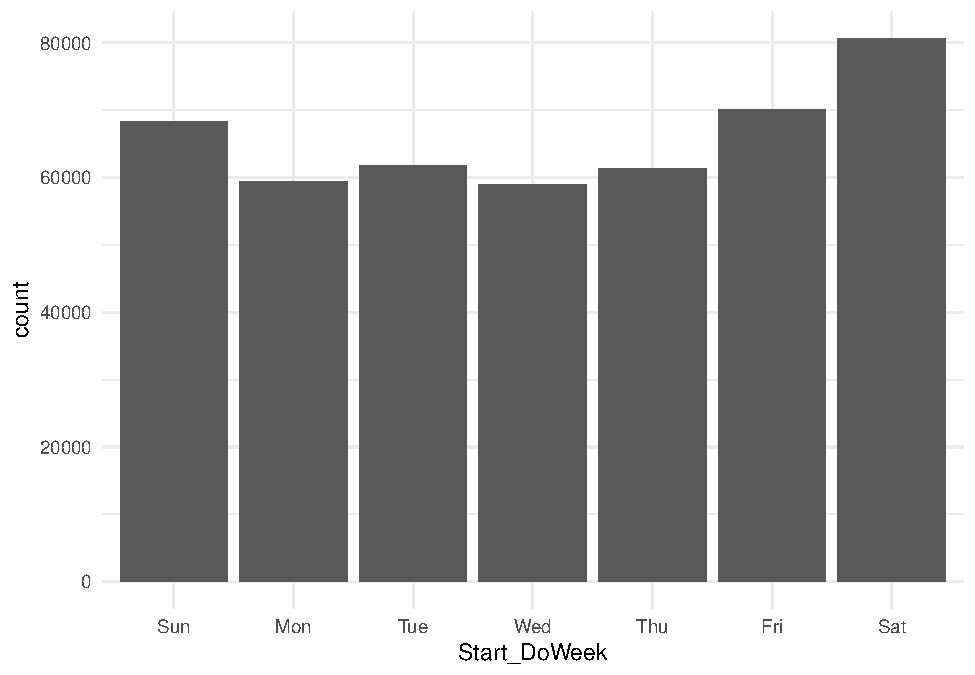
\includegraphics{Nice_Ride_Project_Stat_ReportDRAFT_files/figure-latex/unnamed-chunk-4-1.pdf}

The greatest trip volume is on Saturday, followed by Friday and Sunday.
The lowest trip volume is on Wednesday during the workweek, perhaps
riders that use the bike share for commuting to and from work use other
transportation in the middle of the work week?

\subsubsection{Distribution of trips by day of the week by account
type}\label{distribution-of-trips-by-day-of-the-week-by-account-type}

\begin{Shaded}
\begin{Highlighting}[]
\NormalTok{Rides }\OperatorTok\StringTok{ }\KeywordTok{ggplot}\NormalTok{(}\KeywordTok{aes}\NormalTok{(}\DataTypeTok{x =}\NormalTok{ Start_DoWeek)) }\OperatorTok{+}\StringTok{ }\KeywordTok{geom_bar}\NormalTok{() }\OperatorTok{+}\StringTok{ }\KeywordTok{facet_grid}\NormalTok{(}\OperatorTok{~}\StringTok{ }\NormalTok{Account_Type)}
\end{Highlighting}
\end{Shaded}

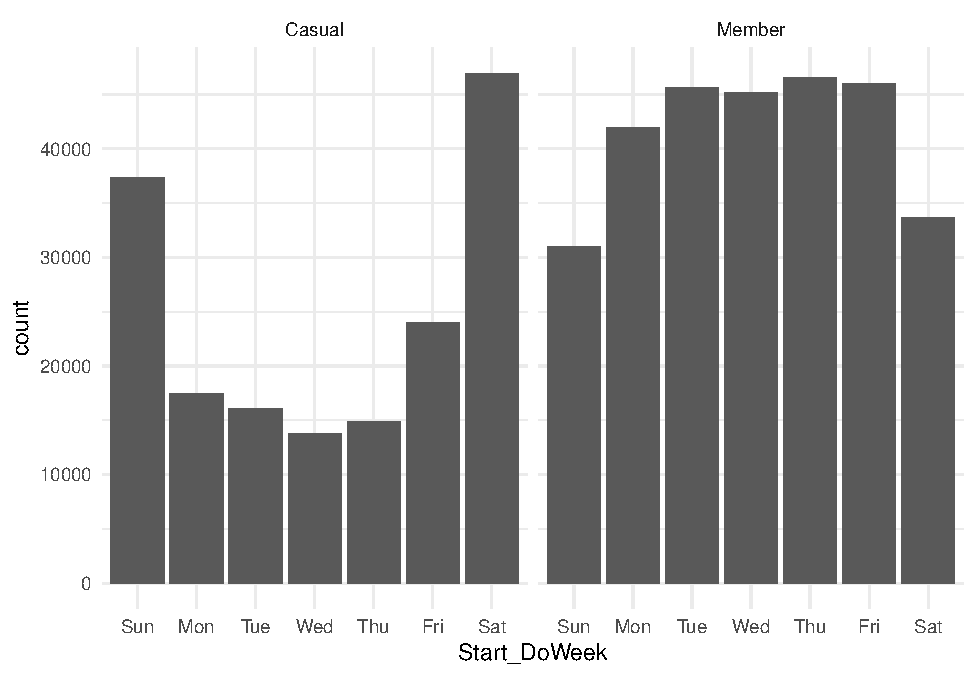
\includegraphics{Nice_Ride_Project_Stat_ReportDRAFT_files/figure-latex/unnamed-chunk-5-1.pdf}

Member trips occur more often on weekdays, likely due to work commutes,
while casual trips occur on the weekends.

\subsubsection{Distribution of trips by hour of weekdays and weekends by
account
type}\label{distribution-of-trips-by-hour-of-weekdays-and-weekends-by-account-type}

\begin{Shaded}
\begin{Highlighting}[]
\NormalTok{Rides }\OperatorTok\StringTok{ }\KeywordTok{ggplot}\NormalTok{(}\KeywordTok{aes}\NormalTok{(Start_Hour)) }\OperatorTok{+}\StringTok{ }\KeywordTok{geom_bar}\NormalTok{() }\OperatorTok{+}\StringTok{ }\KeywordTok{facet_wrap}\NormalTok{(Account_Type }\OperatorTok{~}\StringTok{ }\NormalTok{StartWeek_Day_End, }\DataTypeTok{scales =} \StringTok{"free"}\NormalTok{) }\OperatorTok{+}\StringTok{ }\KeywordTok{scale_x_continuous}\NormalTok{(}\DataTypeTok{breaks =} \KeywordTok{seq}\NormalTok{(}\DecValTok{0}\NormalTok{, }\DecValTok{23}\NormalTok{, }\DataTypeTok{by =} \DecValTok{2}\NormalTok{))}
\end{Highlighting}
\end{Shaded}

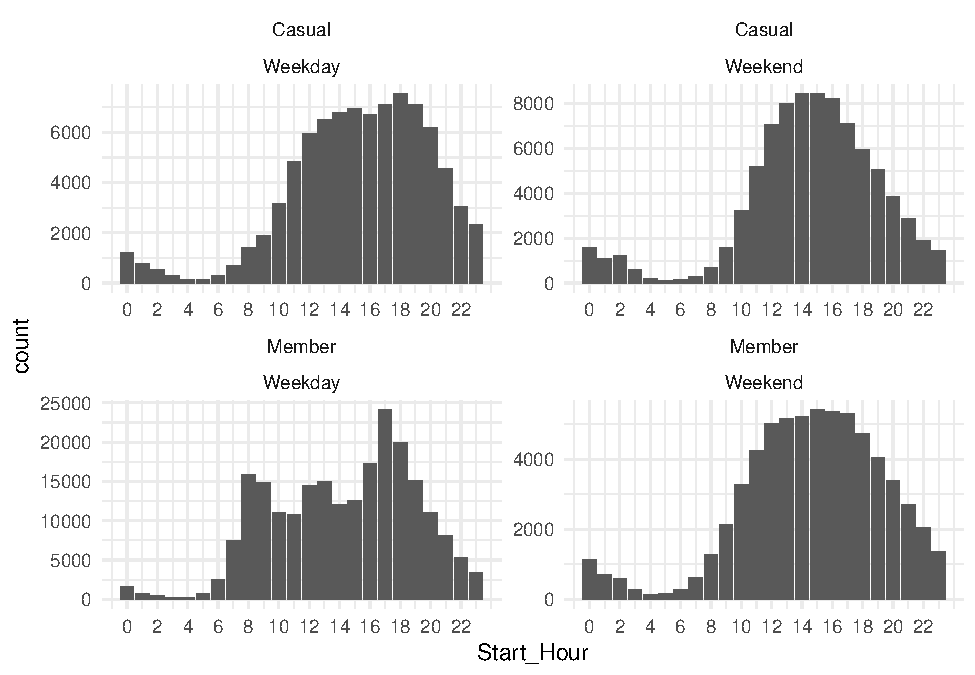
\includegraphics{Nice_Ride_Project_Stat_ReportDRAFT_files/figure-latex/unnamed-chunk-6-1.pdf}

Separating weekdays and weekends confirms the surge in trip volume
during the end of the workday between 5 - 6 PM. Factoring weekday and
weekend also shows the surge in work commutes from 7 - 10 AM on the
weekdays. The weekend shows a pattern of more trips taken from 12 - 7
PM.

\subsection{Observing bike trip duration and distance
variables}\label{observing-bike-trip-duration-and-distance-variables}

\subsubsection{Mean duration of trip by day of
week}\label{mean-duration-of-trip-by-day-of-week}

\begin{Shaded}
\begin{Highlighting}[]
\NormalTok{Rides }\OperatorTok\StringTok{ }\KeywordTok{group_by}\NormalTok{(Start_DoWeek, Account_Type) }\OperatorTok\StringTok{ }\KeywordTok{summarise}\NormalTok{(}\DataTypeTok{Total_DurationMin =} \KeywordTok{mean}\NormalTok{(Total_DurationMin)) }\OperatorTok\StringTok{ }\KeywordTok{ggplot}\NormalTok{(}\KeywordTok{aes}\NormalTok{(Start_DoWeek, Total_DurationMin)) }\OperatorTok{+}\StringTok{ }\KeywordTok{geom_bar}\NormalTok{(}\DataTypeTok{stat =} \StringTok{"identity"}\NormalTok{) }\OperatorTok{+}\StringTok{ }\KeywordTok{facet_wrap}\NormalTok{(}\OperatorTok{~}\StringTok{ }\NormalTok{Account_Type)}
\end{Highlighting}
\end{Shaded}

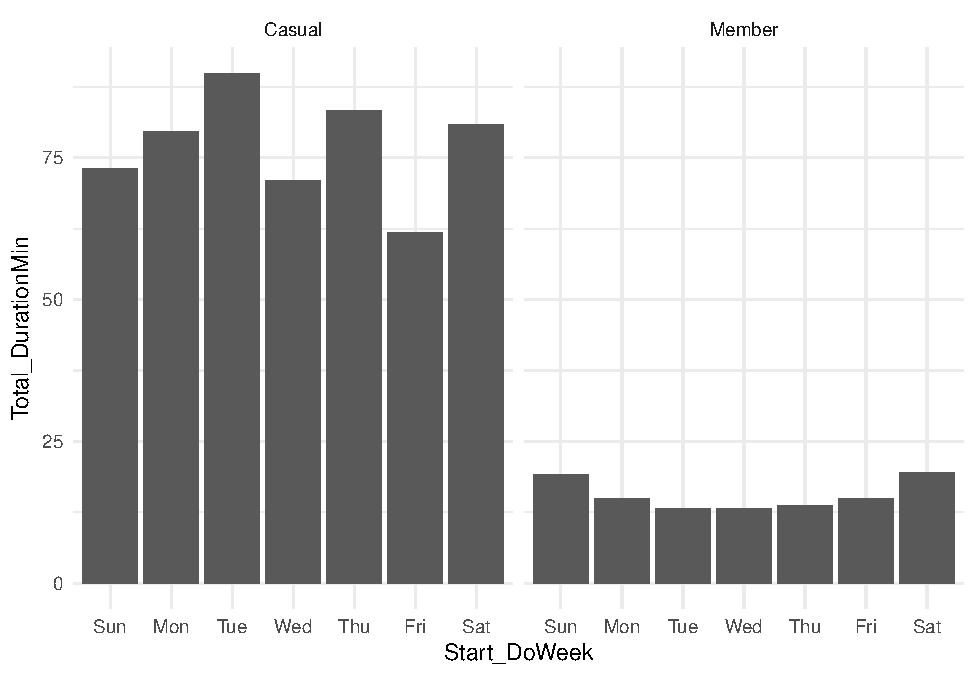
\includegraphics{Nice_Ride_Project_Stat_ReportDRAFT_files/figure-latex/unnamed-chunk-7-1.pdf}

Casual trips have a less uniform distribution of the mean trip duration
per day, while member trips have a more bowl-shaped distribution from
Sunday - Saturday. The mean for member trips is under 25 minutes on all
seven days of the week, while the mean for casual trips is between
60-75+ minutes each day. \emph{Should we question the integrity of our
dataset from this perspective? Do we have outliers to address?}

\subsubsection{Median duration of trip by day of
week}\label{median-duration-of-trip-by-day-of-week}

\begin{Shaded}
\begin{Highlighting}[]
\NormalTok{Rides }\OperatorTok\StringTok{ }\KeywordTok{group_by}\NormalTok{(Start_DoWeek, Account_Type) }\OperatorTok\StringTok{ }\KeywordTok{summarise}\NormalTok{(}\DataTypeTok{Total_DurationMin =} \KeywordTok{median}\NormalTok{(Total_DurationMin)) }\OperatorTok\StringTok{ }\KeywordTok{ggplot}\NormalTok{(}\KeywordTok{aes}\NormalTok{(Start_DoWeek, Total_DurationMin)) }\OperatorTok{+}\StringTok{ }\KeywordTok{geom_bar}\NormalTok{(}\DataTypeTok{stat =} \StringTok{"identity"}\NormalTok{) }\OperatorTok{+}\StringTok{ }\KeywordTok{facet_wrap}\NormalTok{(}\OperatorTok{~}\StringTok{ }\NormalTok{Account_Type)}
\end{Highlighting}
\end{Shaded}

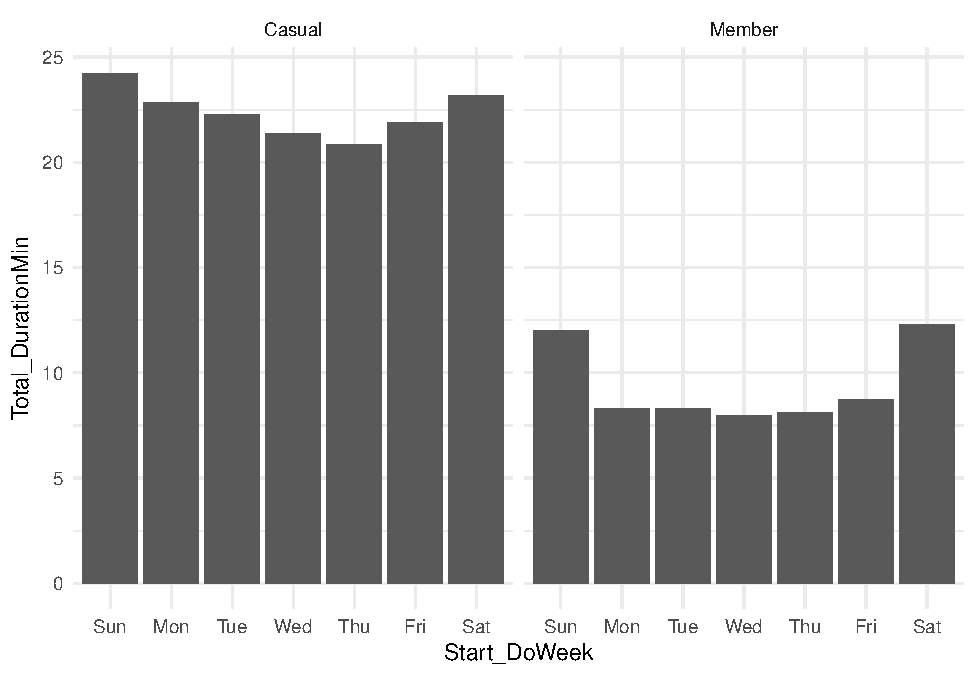
\includegraphics{Nice_Ride_Project_Stat_ReportDRAFT_files/figure-latex/unnamed-chunk-8-1.pdf}

Visualizing the median trip duration by day for casual and member
account types shows that we have outliers in our dataset to address. The
median trip duration for a casual rider is between 20-25 minutes with a
similar bowl-shaped distribution for the week. Member riders maintain a
similar bowl-shaped distribution and have a median trip duration ranging
from 7.5-12.5 minutes depending on the day. \emph{This confirms we have
outliers to address prior further analysis.}

\subsubsection{Mean distance of trip by day of
week}\label{mean-distance-of-trip-by-day-of-week}

\begin{Shaded}
\begin{Highlighting}[]
\NormalTok{Rides }\OperatorTok\StringTok{ }\KeywordTok{group_by}\NormalTok{(Start_DoWeek, Account_Type) }\OperatorTok\StringTok{ }\KeywordTok{summarise}\NormalTok{(}\DataTypeTok{Trip_DistanceMiles =} \KeywordTok{mean}\NormalTok{(Trip_DistanceMiles)) }\OperatorTok\StringTok{ }\KeywordTok{ggplot}\NormalTok{(}\KeywordTok{aes}\NormalTok{(Start_DoWeek, Trip_DistanceMiles)) }\OperatorTok{+}\StringTok{ }\KeywordTok{geom_bar}\NormalTok{(}\DataTypeTok{stat =} \StringTok{"identity"}\NormalTok{) }\OperatorTok{+}\StringTok{ }\KeywordTok{facet_wrap}\NormalTok{(}\OperatorTok{~}\StringTok{ }\NormalTok{Account_Type) }\OperatorTok{+}\StringTok{ }\KeywordTok{scale_y_continuous}\NormalTok{(}\DataTypeTok{breaks =} \KeywordTok{seq}\NormalTok{(}\DecValTok{0}\NormalTok{, }\DecValTok{5}\NormalTok{, }\DataTypeTok{by =} \FloatTok{0.25}\NormalTok{))}
\end{Highlighting}
\end{Shaded}

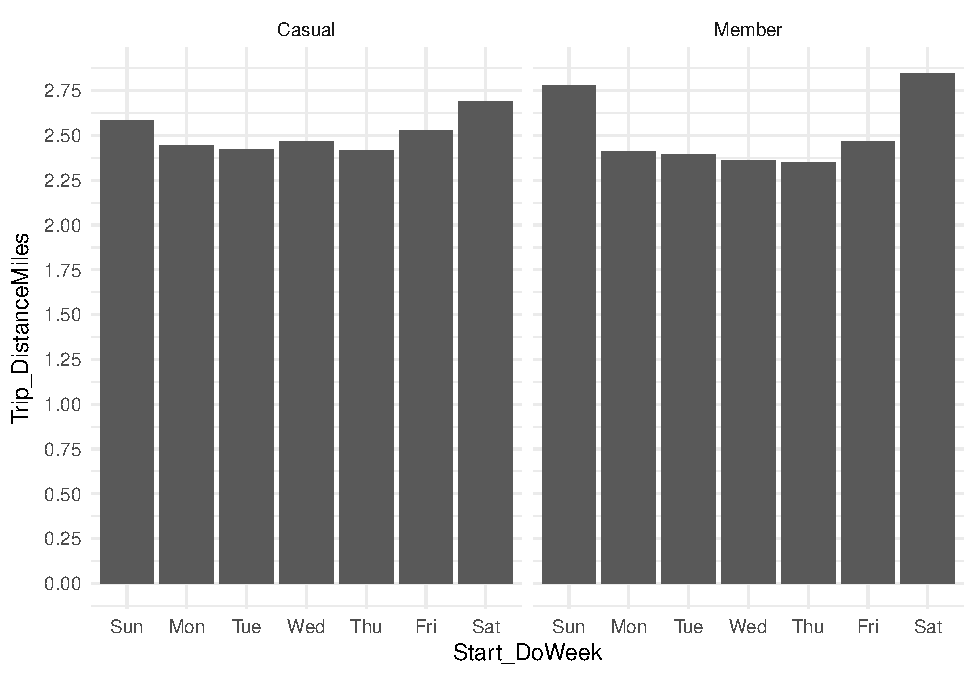
\includegraphics{Nice_Ride_Project_Stat_ReportDRAFT_files/figure-latex/unnamed-chunk-9-1.pdf}

The mean trip distance in miles per day sorted by account type shows a
similar distribution as noticed for trip duration, though the casual
trip distances do not seem skewed by outliers as noted for duration.
Casual rides have a mean range between 2.25 and 2.75 miles depending on
the day, while member account types have a wider range from 2.25 to 3
miles.

\subsubsection{Median distance of trip by day of
week}\label{median-distance-of-trip-by-day-of-week}

\begin{Shaded}
\begin{Highlighting}[]
\NormalTok{Rides }\OperatorTok\StringTok{ }\KeywordTok{group_by}\NormalTok{(Start_DoWeek, Account_Type) }\OperatorTok\StringTok{ }\KeywordTok{summarise}\NormalTok{(}\DataTypeTok{Trip_DistanceMiles =} \KeywordTok{median}\NormalTok{(Trip_DistanceMiles)) }\OperatorTok\StringTok{ }\KeywordTok{ggplot}\NormalTok{(}\KeywordTok{aes}\NormalTok{(Start_DoWeek, Trip_DistanceMiles)) }\OperatorTok{+}\StringTok{ }\KeywordTok{geom_bar}\NormalTok{(}\DataTypeTok{stat =} \StringTok{"identity"}\NormalTok{) }\OperatorTok{+}\StringTok{ }\KeywordTok{facet_wrap}\NormalTok{(}\OperatorTok{~}\StringTok{ }\NormalTok{Account_Type) }\OperatorTok{+}\StringTok{ }\KeywordTok{scale_y_continuous}\NormalTok{(}\DataTypeTok{breaks =} \KeywordTok{seq}\NormalTok{(}\DecValTok{0}\NormalTok{, }\DecValTok{5}\NormalTok{, }\DataTypeTok{by =} \FloatTok{0.25}\NormalTok{))}
\end{Highlighting}
\end{Shaded}

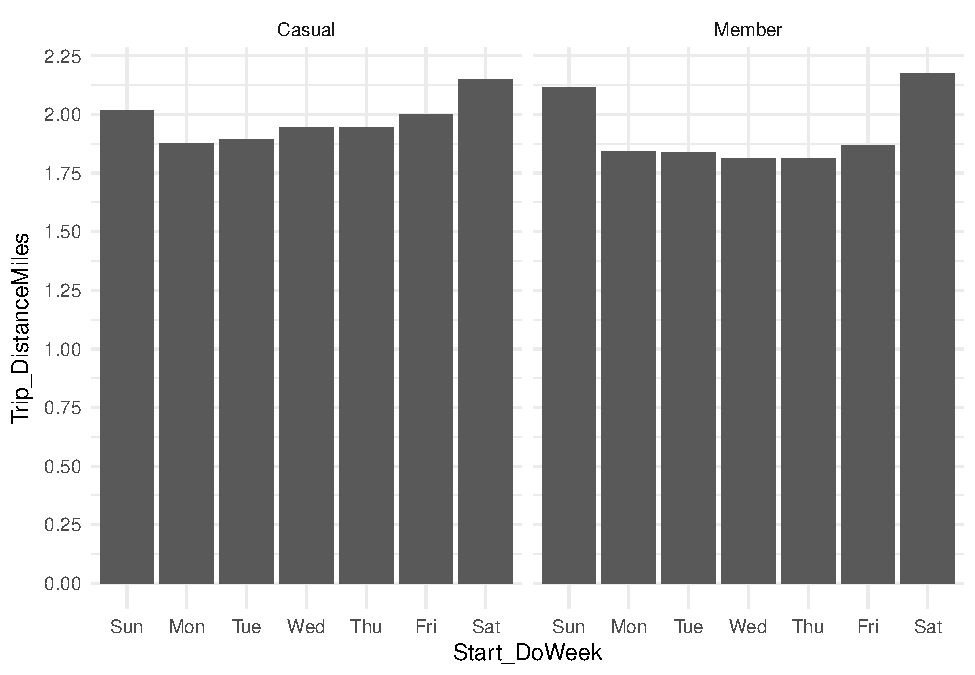
\includegraphics{Nice_Ride_Project_Stat_ReportDRAFT_files/figure-latex/unnamed-chunk-10-1.pdf}

The median trip distance in miles per day holds a similar result to the
mean distance, though the range per day is shorter with casual and
member account falling in the same range of 1.75 to 2.25 miles.

\subsection{Observing weather variable affects on bike
use}\label{observing-weather-variable-affects-on-bike-use}

\subsubsection{How does temperature affect bike
use?}\label{how-does-temperature-affect-bike-use}

\begin{Shaded}
\begin{Highlighting}[]
\CommentTok{#Distribution of trips in relation to temperature by weekday and weekend}
\NormalTok{Rides }\OperatorTok\StringTok{ }\KeywordTok{ggplot}\NormalTok{(}\KeywordTok{aes}\NormalTok{(Temp_F)) }\OperatorTok{+}\StringTok{ }\KeywordTok{geom_density}\NormalTok{() }\OperatorTok{+}\StringTok{ }\KeywordTok{facet_wrap}\NormalTok{(}\OperatorTok{~}\StringTok{ }\NormalTok{StartWeek_Day_End) }\OperatorTok{+}\StringTok{ }\KeywordTok{scale_x_continuous}\NormalTok{(}\DataTypeTok{breaks =} \KeywordTok{seq}\NormalTok{(}\DecValTok{0}\NormalTok{, }\DecValTok{100}\NormalTok{, }\DataTypeTok{by =} \DecValTok{5}\NormalTok{))}
\end{Highlighting}
\end{Shaded}

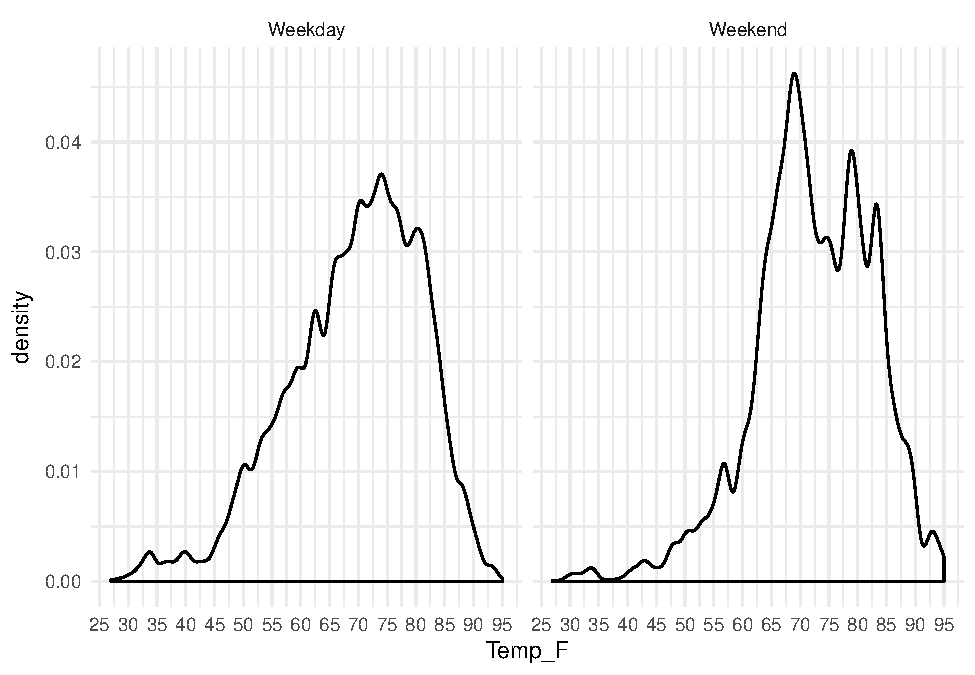
\includegraphics{Nice_Ride_Project_Stat_ReportDRAFT_files/figure-latex/unnamed-chunk-11-1.pdf}

\begin{Shaded}
\begin{Highlighting}[]
\CommentTok{#Distribution of trips in relation temperature by member or casual}
\NormalTok{Rides }\OperatorTok\StringTok{ }\KeywordTok{ggplot}\NormalTok{(}\KeywordTok{aes}\NormalTok{(Temp_F)) }\OperatorTok{+}\StringTok{ }\KeywordTok{geom_density}\NormalTok{() }\OperatorTok{+}\StringTok{ }\KeywordTok{facet_wrap}\NormalTok{(}\OperatorTok{~}\StringTok{ }\NormalTok{Account_Type) }\OperatorTok{+}\StringTok{ }\KeywordTok{scale_x_continuous}\NormalTok{(}\DataTypeTok{breaks =} \KeywordTok{seq}\NormalTok{(}\DecValTok{0}\NormalTok{, }\DecValTok{100}\NormalTok{, }\DataTypeTok{by =} \DecValTok{5}\NormalTok{)) }
\end{Highlighting}
\end{Shaded}

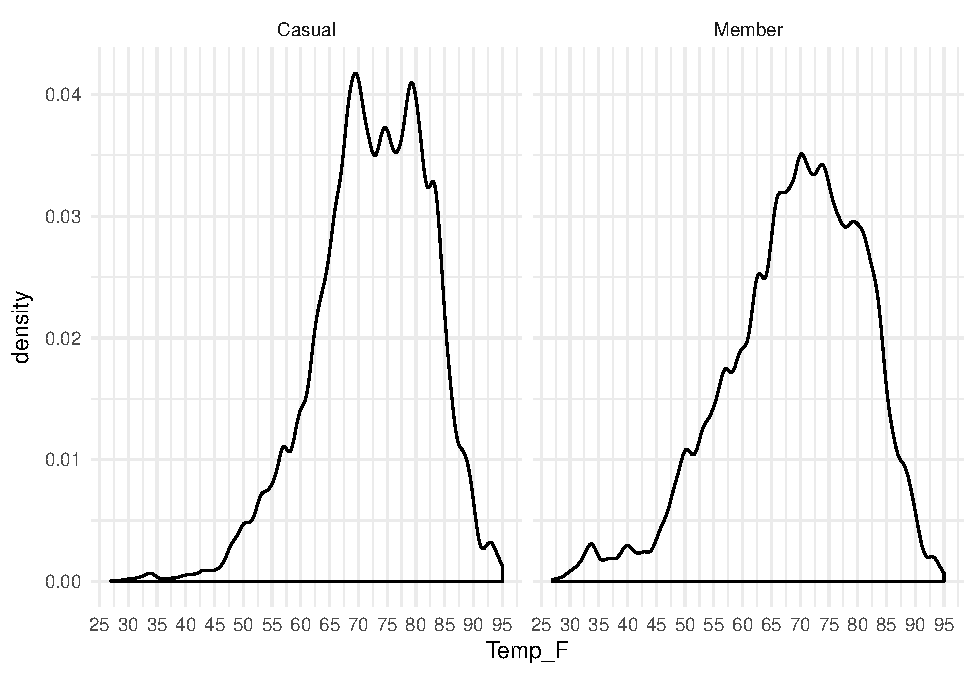
\includegraphics{Nice_Ride_Project_Stat_ReportDRAFT_files/figure-latex/unnamed-chunk-11-2.pdf}

\begin{Shaded}
\begin{Highlighting}[]
\CommentTok{#Distribution of trips in relation to temperature by weekday and weekend and member or casual}
\NormalTok{Rides }\OperatorTok\StringTok{ }\KeywordTok{ggplot}\NormalTok{(}\KeywordTok{aes}\NormalTok{(Temp_F)) }\OperatorTok{+}\StringTok{ }\KeywordTok{geom_density}\NormalTok{() }\OperatorTok{+}\StringTok{ }\KeywordTok{facet_wrap}\NormalTok{(Account_Type }\OperatorTok{~}\StringTok{ }\NormalTok{StartWeek_Day_End, }\DataTypeTok{scale =} \StringTok{"free"}\NormalTok{) }\OperatorTok{+}\StringTok{ }\KeywordTok{scale_x_continuous}\NormalTok{(}\DataTypeTok{breaks =} \KeywordTok{seq}\NormalTok{(}\DecValTok{0}\NormalTok{, }\DecValTok{100}\NormalTok{, }\DataTypeTok{by =} \DecValTok{5}\NormalTok{)) }
\end{Highlighting}
\end{Shaded}

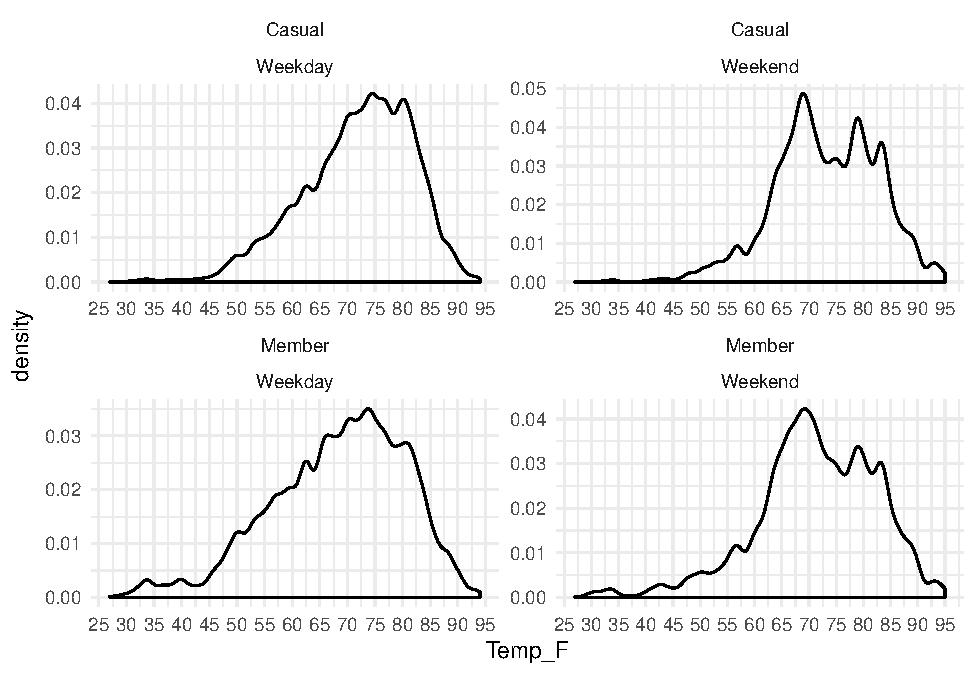
\includegraphics{Nice_Ride_Project_Stat_ReportDRAFT_files/figure-latex/unnamed-chunk-11-3.pdf}

Visualizing weekday and weekend trips by account type in relation to the
dry bulb temperature in Fahrenheit reading shows similarity between
casual and member riders for weekdays and the same for weekends. Riders
are willing to use the bike share at a higher range of temperatures
during the weekdays than they are on the weekend. The majority of rides
for weekdays occur between 70 and 82.5 degrees fahrenheit while rides on
weekends peak at 68 degrees and steadily decline there afterward, though
there are increases in volume in the high 70's and low 80's. For colder
temperatures casual riders participate at minimal levels until
temperatures approach the low 50's, while member riders show some bike
share use in cold temperatures and a strong increase starting in the
mid-40's.

\subsubsection{How does precipitation affect bike
use?}\label{how-does-precipitation-affect-bike-use}

\emph{This visualization doesn't quite capture it}

\begin{Shaded}
\begin{Highlighting}[]
\CommentTok{#Distribution of trips in relation to precipitation by weekday and weekend}
\NormalTok{Rides }\OperatorTok\StringTok{ }\KeywordTok{ggplot}\NormalTok{(}\KeywordTok{aes}\NormalTok{(Precipitation, }\DataTypeTok{color =}\NormalTok{ StartWeek_Day_End)) }\OperatorTok{+}\StringTok{ }\KeywordTok{geom_density}\NormalTok{() }\OperatorTok{+}\StringTok{ }\KeywordTok{scale_x_continuous}\NormalTok{(}\DataTypeTok{breaks =} \KeywordTok{seq}\NormalTok{(}\DecValTok{0}\NormalTok{, }\DecValTok{1}\NormalTok{, }\DataTypeTok{by =} \FloatTok{0.10}\NormalTok{))}
\end{Highlighting}
\end{Shaded}

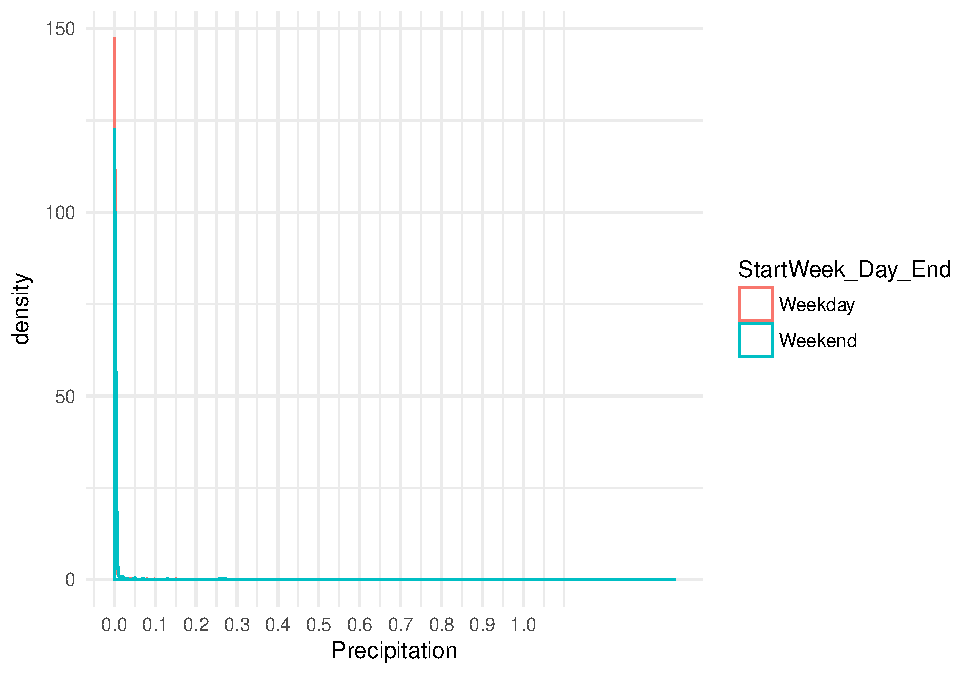
\includegraphics{Nice_Ride_Project_Stat_ReportDRAFT_files/figure-latex/unnamed-chunk-12-1.pdf}

\begin{Shaded}
\begin{Highlighting}[]
\CommentTok{#Distribution of trips in relation to precipitation by member or casual}
\NormalTok{Rides }\OperatorTok\StringTok{ }\KeywordTok{ggplot}\NormalTok{(}\KeywordTok{aes}\NormalTok{(Precipitation, }\DataTypeTok{color =}\NormalTok{ Account_Type)) }\OperatorTok{+}\StringTok{ }\KeywordTok{geom_density}\NormalTok{() }\OperatorTok{+}\StringTok{ }\KeywordTok{scale_x_continuous}\NormalTok{(}\DataTypeTok{breaks =} \KeywordTok{seq}\NormalTok{(}\DecValTok{0}\NormalTok{, }\DecValTok{1}\NormalTok{, }\DataTypeTok{by =} \FloatTok{0.10}\NormalTok{))}
\end{Highlighting}
\end{Shaded}

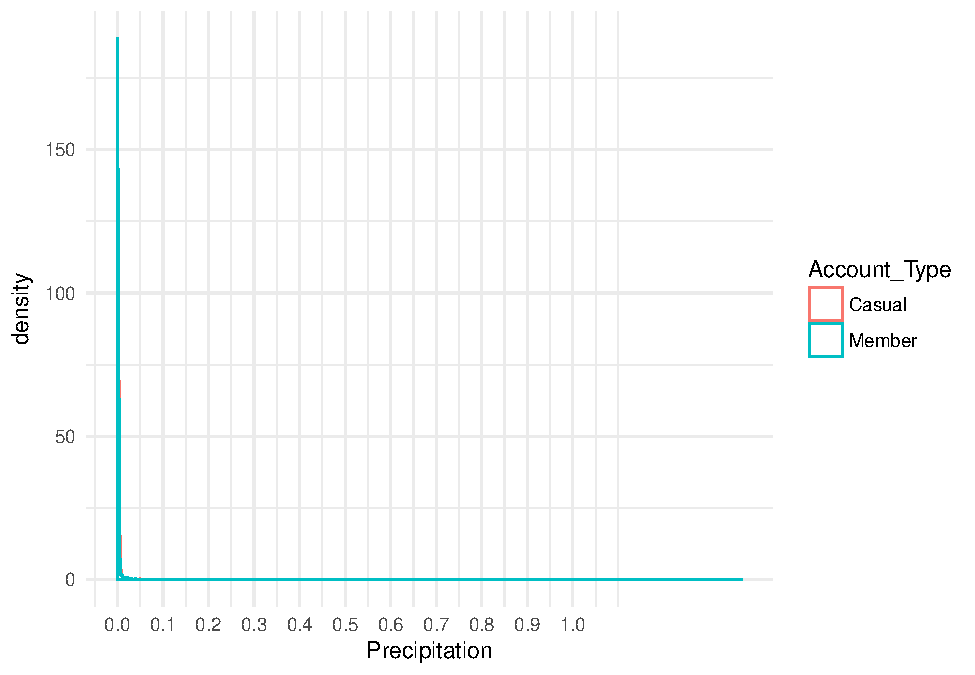
\includegraphics{Nice_Ride_Project_Stat_ReportDRAFT_files/figure-latex/unnamed-chunk-12-2.pdf}

\begin{Shaded}
\begin{Highlighting}[]
\CommentTok{#Distribution of trips in relation to precipitation by weekday and weekend and member or casual}
\NormalTok{Rides }\OperatorTok\StringTok{ }\KeywordTok{ggplot}\NormalTok{(}\KeywordTok{aes}\NormalTok{(Precipitation, }\DataTypeTok{color =}\NormalTok{ StartWeek_Day_End)) }\OperatorTok{+}\StringTok{ }\KeywordTok{geom_density}\NormalTok{() }\OperatorTok{+}\StringTok{ }\KeywordTok{facet_wrap}\NormalTok{(}\OperatorTok{~}\StringTok{ }\NormalTok{Account_Type) }\OperatorTok{+}\StringTok{ }\KeywordTok{scale_x_continuous}\NormalTok{(}\DataTypeTok{breaks =} \KeywordTok{seq}\NormalTok{(}\DecValTok{0}\NormalTok{, }\DecValTok{1}\NormalTok{, }\DataTypeTok{by =} \FloatTok{0.10}\NormalTok{))}
\end{Highlighting}
\end{Shaded}

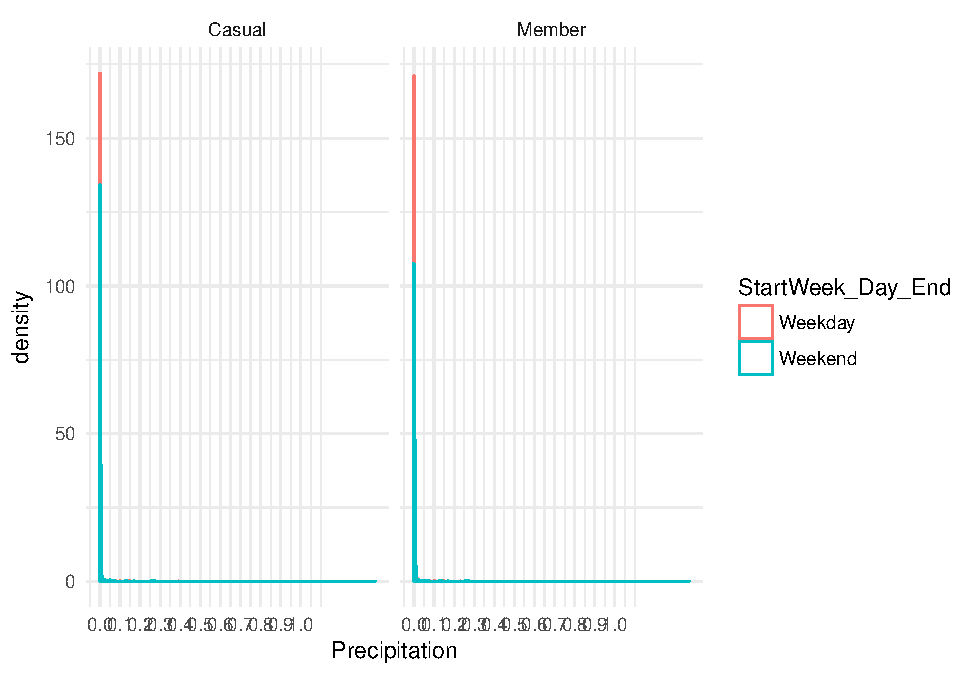
\includegraphics{Nice_Ride_Project_Stat_ReportDRAFT_files/figure-latex/unnamed-chunk-12-3.pdf}

Precipitation play a large factor in bike use for both casual and member
account types and greatly declines for precipitation levels beyond 0.1
inches.

\subsubsection{How does humidity affect bike
use?}\label{how-does-humidity-affect-bike-use}

\begin{Shaded}
\begin{Highlighting}[]
\CommentTok{#Distribution of trips in relation to humidity by weekday and weekend}
\NormalTok{Rides }\OperatorTok\StringTok{ }\KeywordTok{ggplot}\NormalTok{(}\KeywordTok{aes}\NormalTok{(Rel_Humidity, }\DataTypeTok{color =}\NormalTok{ StartWeek_Day_End)) }\OperatorTok{+}\StringTok{ }\KeywordTok{geom_density}\NormalTok{() }\OperatorTok{+}\StringTok{ }\KeywordTok{scale_x_continuous}\NormalTok{(}\DataTypeTok{breaks =} \KeywordTok{seq}\NormalTok{(}\DecValTok{0}\NormalTok{, }\DecValTok{100}\NormalTok{, }\DataTypeTok{by =} \DecValTok{10}\NormalTok{)) }
\end{Highlighting}
\end{Shaded}

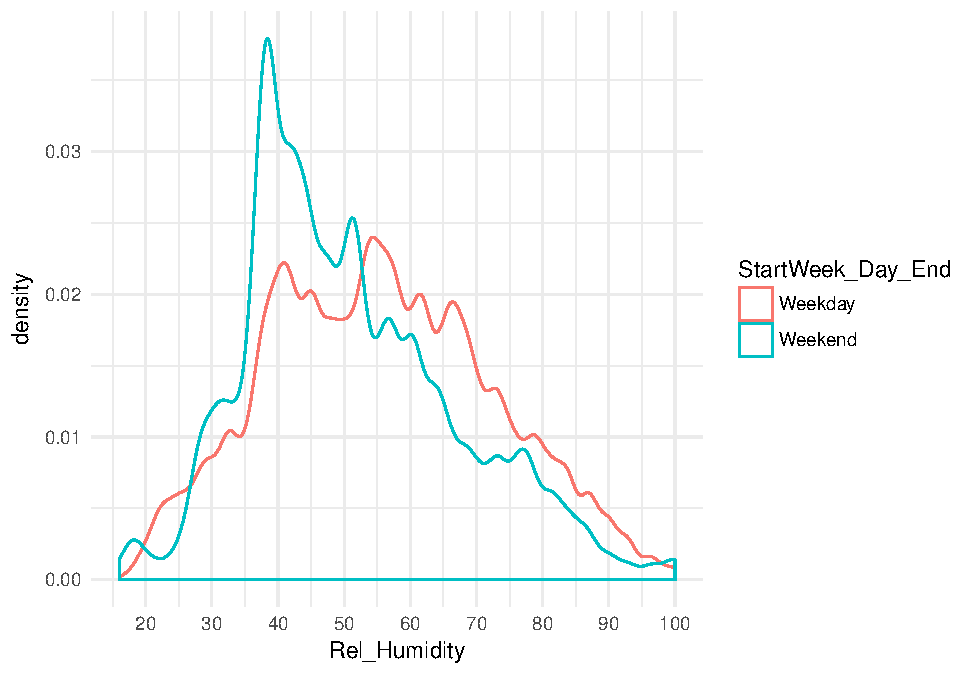
\includegraphics{Nice_Ride_Project_Stat_ReportDRAFT_files/figure-latex/unnamed-chunk-13-1.pdf}

\begin{Shaded}
\begin{Highlighting}[]
\CommentTok{#Distribution of trips in relation humidity by member or casual}
\NormalTok{Rides }\OperatorTok\StringTok{ }\KeywordTok{ggplot}\NormalTok{(}\KeywordTok{aes}\NormalTok{(Rel_Humidity, }\DataTypeTok{color =}\NormalTok{ Account_Type)) }\OperatorTok{+}\StringTok{ }\KeywordTok{geom_density}\NormalTok{() }\OperatorTok{+}\StringTok{ }\KeywordTok{scale_x_continuous}\NormalTok{(}\DataTypeTok{breaks =} \KeywordTok{seq}\NormalTok{(}\DecValTok{0}\NormalTok{, }\DecValTok{100}\NormalTok{, }\DataTypeTok{by =} \DecValTok{10}\NormalTok{)) }
\end{Highlighting}
\end{Shaded}

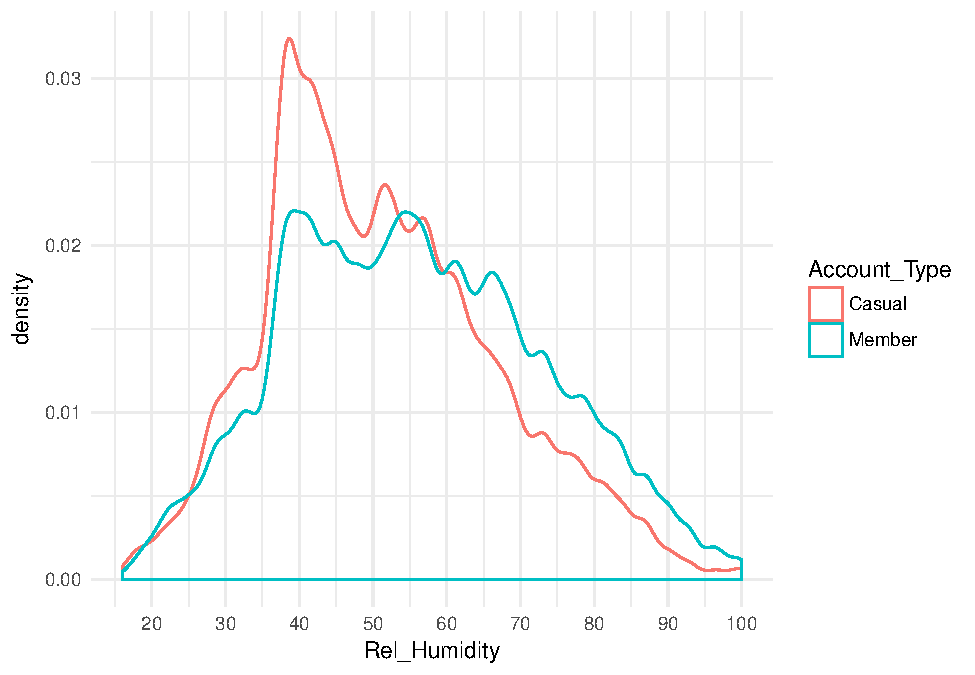
\includegraphics{Nice_Ride_Project_Stat_ReportDRAFT_files/figure-latex/unnamed-chunk-13-2.pdf}

\begin{Shaded}
\begin{Highlighting}[]
\CommentTok{#Distribution of trips in relation to humidity by weekday and weekend and member or casual}
\NormalTok{Rides }\OperatorTok\StringTok{ }\KeywordTok{ggplot}\NormalTok{(}\KeywordTok{aes}\NormalTok{(Rel_Humidity, }\DataTypeTok{color =}\NormalTok{ StartWeek_Day_End)) }\OperatorTok{+}\StringTok{ }\KeywordTok{geom_density}\NormalTok{() }\OperatorTok{+}\StringTok{ }\KeywordTok{facet_wrap}\NormalTok{(}\OperatorTok{~}\StringTok{ }\NormalTok{Account_Type) }\OperatorTok{+}\StringTok{ }\KeywordTok{scale_x_continuous}\NormalTok{(}\DataTypeTok{breaks =} \KeywordTok{seq}\NormalTok{(}\DecValTok{0}\NormalTok{, }\DecValTok{100}\NormalTok{, }\DataTypeTok{by =} \DecValTok{10}\NormalTok{)) }
\end{Highlighting}
\end{Shaded}

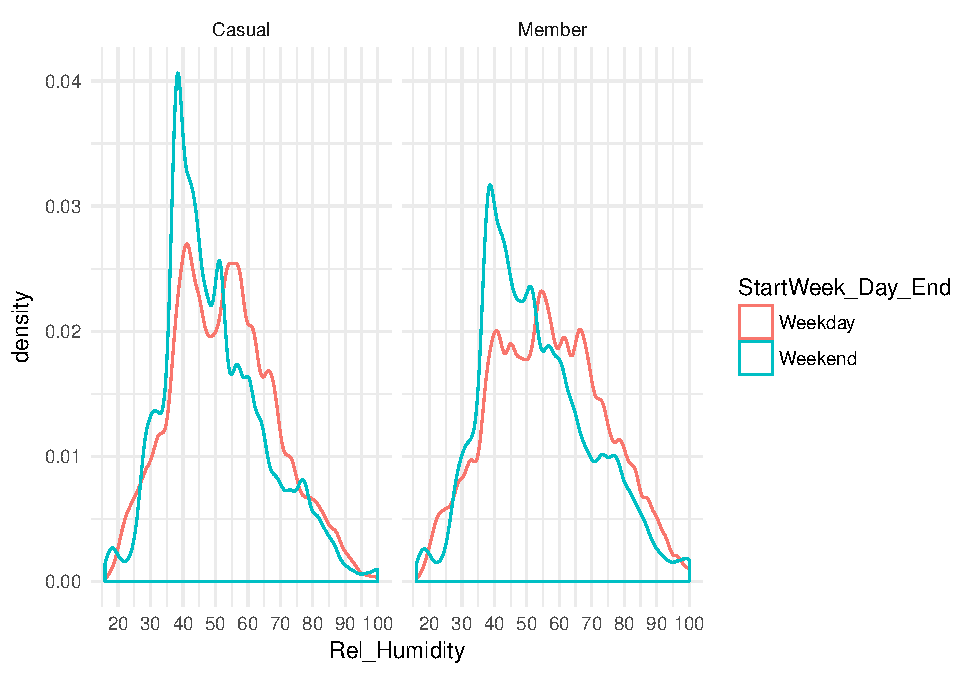
\includegraphics{Nice_Ride_Project_Stat_ReportDRAFT_files/figure-latex/unnamed-chunk-13-3.pdf}

As relative humidity increases bike use declines for both account types.
Both casual and member accounts show a comparable response to relative
humidity during the weekday, though casual riders show a faster decline
in bike usage as humidity rises. Weekend patterns show a similar
response to humidity for casual and member riders.

\subsubsection{How does wind speed affect bike
use?}\label{how-does-wind-speed-affect-bike-use}

\begin{Shaded}
\begin{Highlighting}[]
\CommentTok{#Distribution of trips in relation to wind speed by weekday and weekend}
\NormalTok{Rides }\OperatorTok\StringTok{ }\KeywordTok{ggplot}\NormalTok{(}\KeywordTok{aes}\NormalTok{(Wind_Speed, }\DataTypeTok{color =}\NormalTok{ StartWeek_Day_End)) }\OperatorTok{+}\StringTok{ }\KeywordTok{geom_density}\NormalTok{() }\OperatorTok{+}\StringTok{ }\KeywordTok{scale_x_continuous}\NormalTok{(}\DataTypeTok{breaks =} \KeywordTok{seq}\NormalTok{(}\DecValTok{0}\NormalTok{, }\DecValTok{30}\NormalTok{, }\DataTypeTok{by =} \DecValTok{2}\NormalTok{))}
\end{Highlighting}
\end{Shaded}

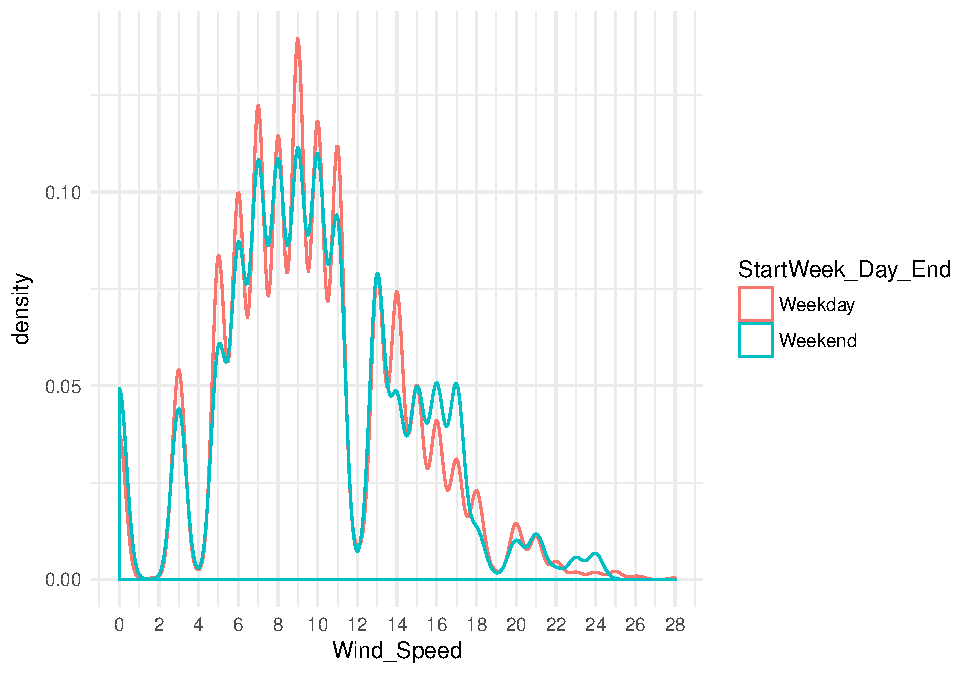
\includegraphics{Nice_Ride_Project_Stat_ReportDRAFT_files/figure-latex/unnamed-chunk-14-1.pdf}

\begin{Shaded}
\begin{Highlighting}[]
\CommentTok{#Distribution of trips in relation to wind speed by member or casual}
\NormalTok{Rides }\OperatorTok\StringTok{ }\KeywordTok{ggplot}\NormalTok{(}\KeywordTok{aes}\NormalTok{(Wind_Speed, }\DataTypeTok{color =}\NormalTok{ Account_Type)) }\OperatorTok{+}\StringTok{ }\KeywordTok{geom_density}\NormalTok{() }\OperatorTok{+}\StringTok{ }\KeywordTok{scale_x_continuous}\NormalTok{(}\DataTypeTok{breaks =} \KeywordTok{seq}\NormalTok{(}\DecValTok{0}\NormalTok{, }\DecValTok{30}\NormalTok{, }\DataTypeTok{by =} \DecValTok{2}\NormalTok{))}
\end{Highlighting}
\end{Shaded}

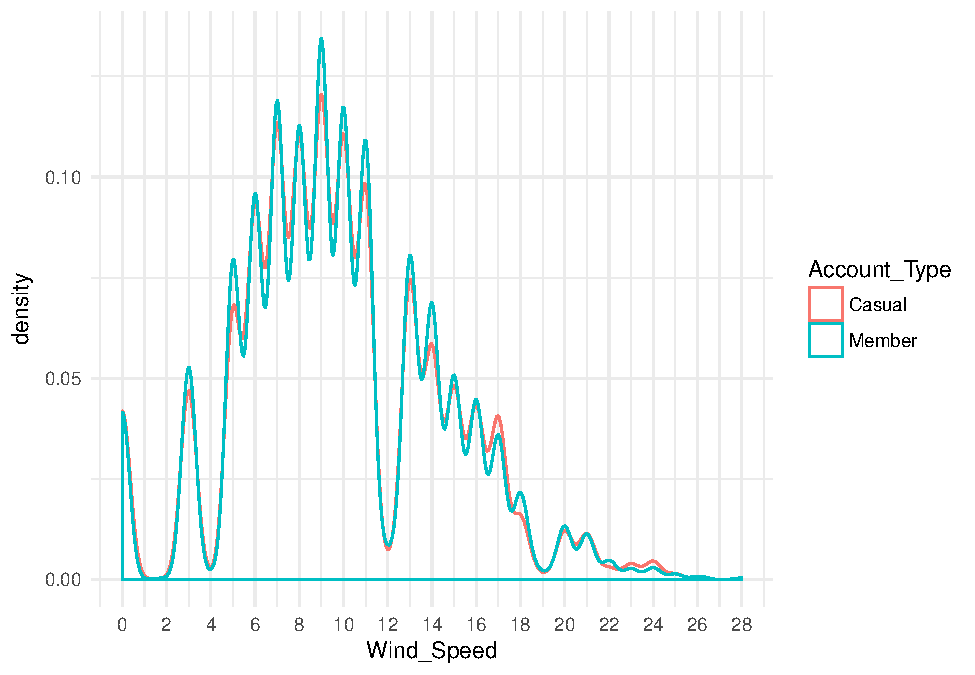
\includegraphics{Nice_Ride_Project_Stat_ReportDRAFT_files/figure-latex/unnamed-chunk-14-2.pdf}

\begin{Shaded}
\begin{Highlighting}[]
\CommentTok{#Distribution of trips in relation to wind speed by weekday and weekend and member or casual}
\NormalTok{Rides }\OperatorTok\StringTok{ }\KeywordTok{ggplot}\NormalTok{(}\KeywordTok{aes}\NormalTok{(Wind_Speed, }\DataTypeTok{color =}\NormalTok{ StartWeek_Day_End)) }\OperatorTok{+}\StringTok{ }\KeywordTok{geom_density}\NormalTok{(}\DataTypeTok{adjust =} \FloatTok{1.25}\NormalTok{) }\OperatorTok{+}\StringTok{ }\KeywordTok{facet_wrap}\NormalTok{(}\OperatorTok{~}\StringTok{ }\NormalTok{Account_Type) }\OperatorTok{+}\StringTok{ }\KeywordTok{scale_x_continuous}\NormalTok{(}\DataTypeTok{breaks =} \KeywordTok{seq}\NormalTok{(}\DecValTok{0}\NormalTok{, }\DecValTok{30}\NormalTok{, }\DataTypeTok{by =} \DecValTok{5}\NormalTok{)) }\OperatorTok{+}\StringTok{ }\KeywordTok{theme}\NormalTok{(}\DataTypeTok{legend.position =} \StringTok{"bottom"}\NormalTok{)}
\end{Highlighting}
\end{Shaded}

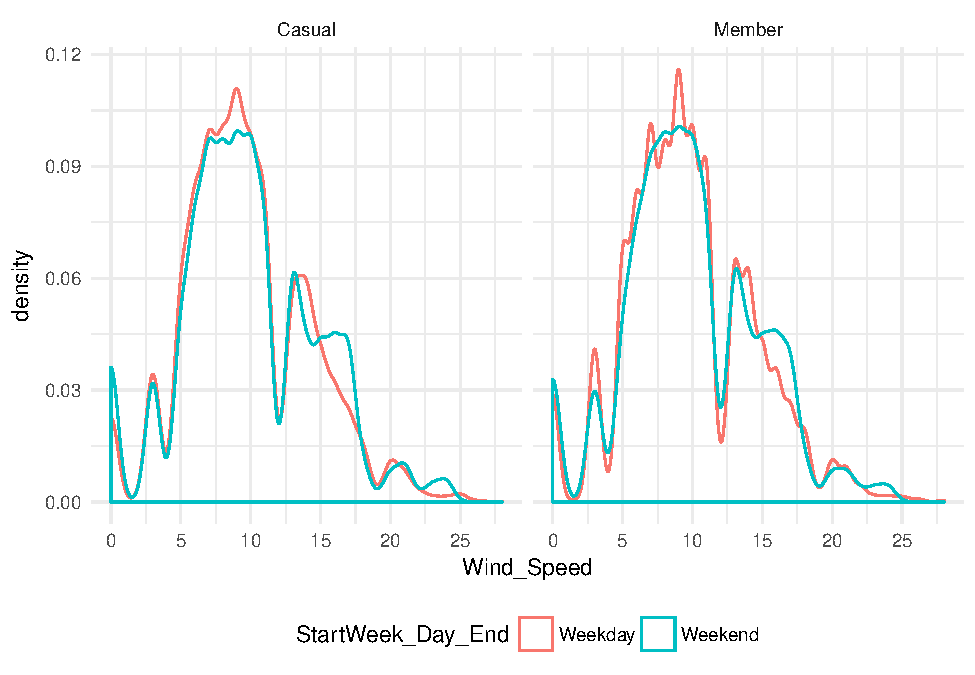
\includegraphics{Nice_Ride_Project_Stat_ReportDRAFT_files/figure-latex/unnamed-chunk-14-3.pdf}

Casual rides show similar responses to an increase in wind speed for
weekday and weekend trips, though there is slightly more tolerance of
riders for wind speeds of 15-17.5 miles per hour on the weekends. Member
riders show a very similar response.

\subsubsection{How does heat index affect bike
use?}\label{how-does-heat-index-affect-bike-use}

\begin{Shaded}
\begin{Highlighting}[]
\CommentTok{#Distribution of trips in relation to heat index by weekday and weekend}
\KeywordTok{ggplot}\NormalTok{(Rides, }\KeywordTok{aes}\NormalTok{(Heat_Index, }\DataTypeTok{color =}\NormalTok{ StartWeek_Day_End)) }\OperatorTok{+}\StringTok{ }\KeywordTok{geom_density}\NormalTok{()}
\end{Highlighting}
\end{Shaded}

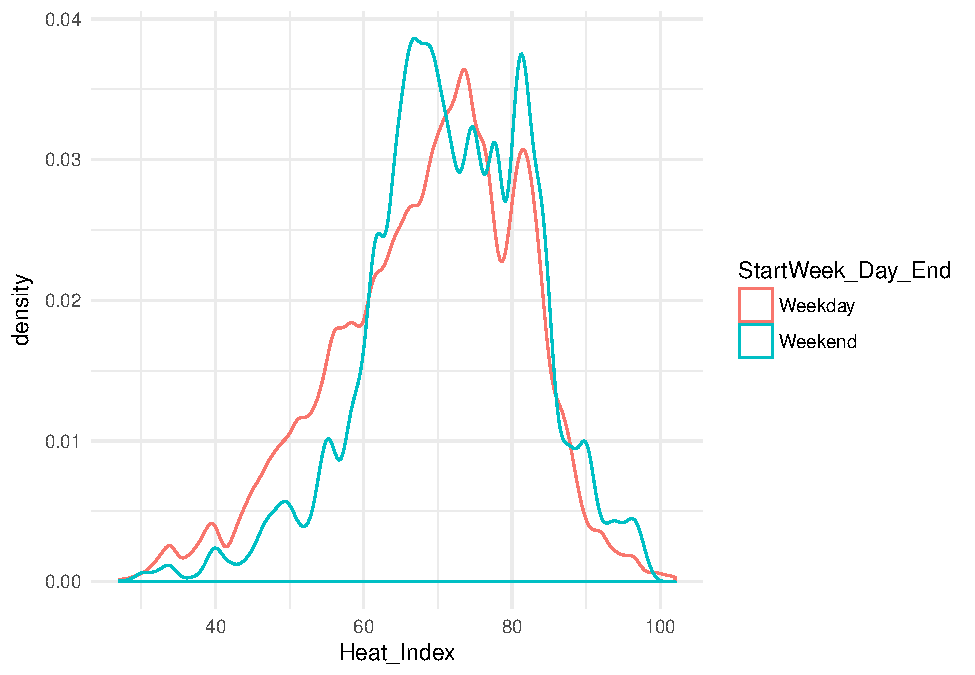
\includegraphics{Nice_Ride_Project_Stat_ReportDRAFT_files/figure-latex/unnamed-chunk-15-1.pdf}

\begin{Shaded}
\begin{Highlighting}[]
\CommentTok{#Distribution of trips in relation to wind speed by member or casual}
\KeywordTok{ggplot}\NormalTok{(Rides, }\KeywordTok{aes}\NormalTok{(Heat_Index, }\DataTypeTok{color =}\NormalTok{ Account_Type)) }\OperatorTok{+}\StringTok{ }\KeywordTok{geom_density}\NormalTok{()}
\end{Highlighting}
\end{Shaded}

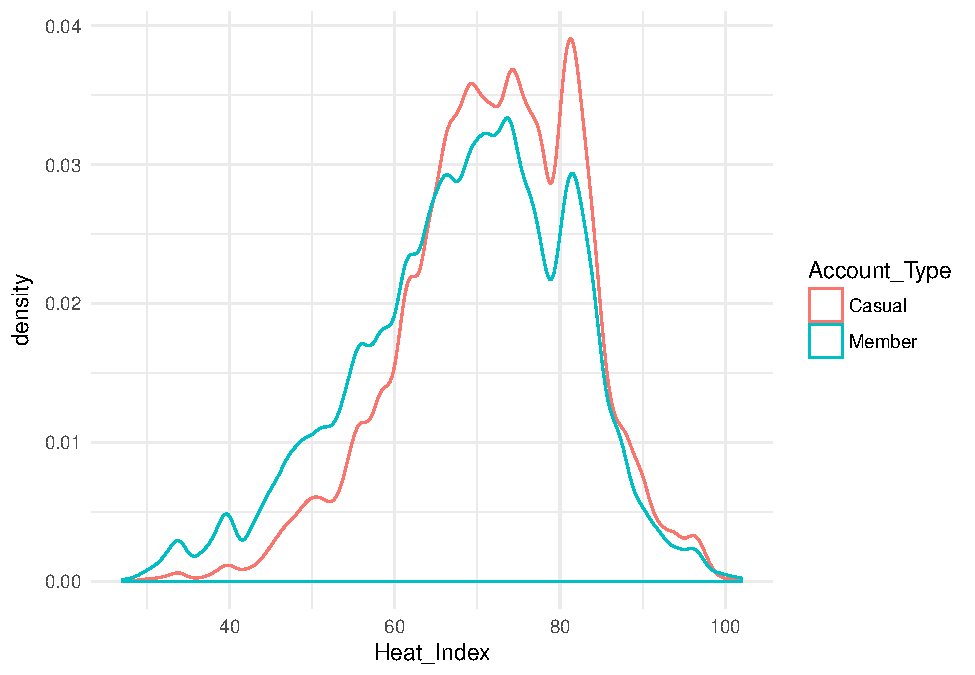
\includegraphics{Nice_Ride_Project_Stat_ReportDRAFT_files/figure-latex/unnamed-chunk-15-2.pdf}

\begin{Shaded}
\begin{Highlighting}[]
\CommentTok{#Distribution of trips in relation to wind speed by weekday and weekend and member or casual}
\KeywordTok{ggplot}\NormalTok{(Rides, }\KeywordTok{aes}\NormalTok{(Heat_Index, }\DataTypeTok{color =}\NormalTok{ StartWeek_Day_End)) }\OperatorTok{+}\StringTok{ }\KeywordTok{geom_density}\NormalTok{() }\OperatorTok{+}\StringTok{ }\KeywordTok{facet_wrap}\NormalTok{(}\OperatorTok{~}\StringTok{ }\NormalTok{Account_Type)}
\end{Highlighting}
\end{Shaded}

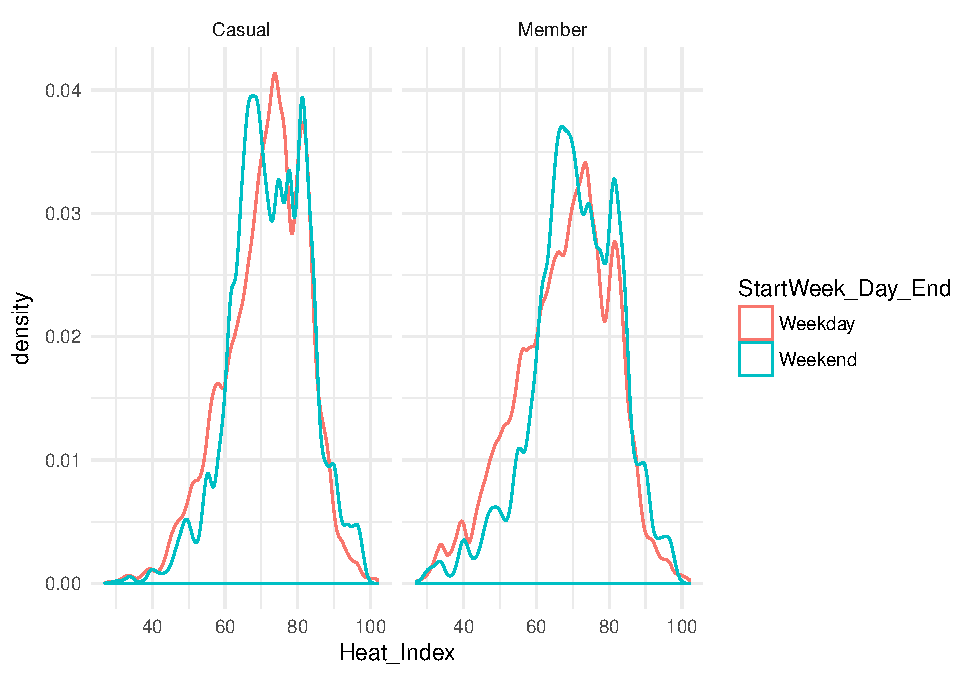
\includegraphics{Nice_Ride_Project_Stat_ReportDRAFT_files/figure-latex/unnamed-chunk-15-3.pdf}

The heat index - variable combining temperature and relative humidity -
holds comparable responses in rider volumes for casual and member
account types. Riders of both account types are more tolerant of a low
heat index on the weekdays and a higher heat index on the weekends. Both
casual and member rides drop severely as the heat index increases above
the low 80's, as to be expected.

\subsection{Time Series Plots}\label{time-series-plots}

\textbf{DOES NOT WORK CORRECTLY DUE TO DISCRETE OBSERVATIONS AND THE
SEPARATION OF DATE/TIME VARIABLES? HOW TO ADDRESS THIS?}

\begin{Shaded}
\begin{Highlighting}[]
\NormalTok{Rides }\OperatorTok\StringTok{ }\KeywordTok{ggplot}\NormalTok{(}\KeywordTok{aes}\NormalTok{(Start_Day, Total_DurationMin)) }\OperatorTok{+}\StringTok{ }\KeywordTok{geom_point}\NormalTok{() }\OperatorTok{+}\StringTok{ }\KeywordTok{facet_wrap}\NormalTok{(}\OperatorTok{~}\StringTok{ }\NormalTok{Start_Month)}
\end{Highlighting}
\end{Shaded}

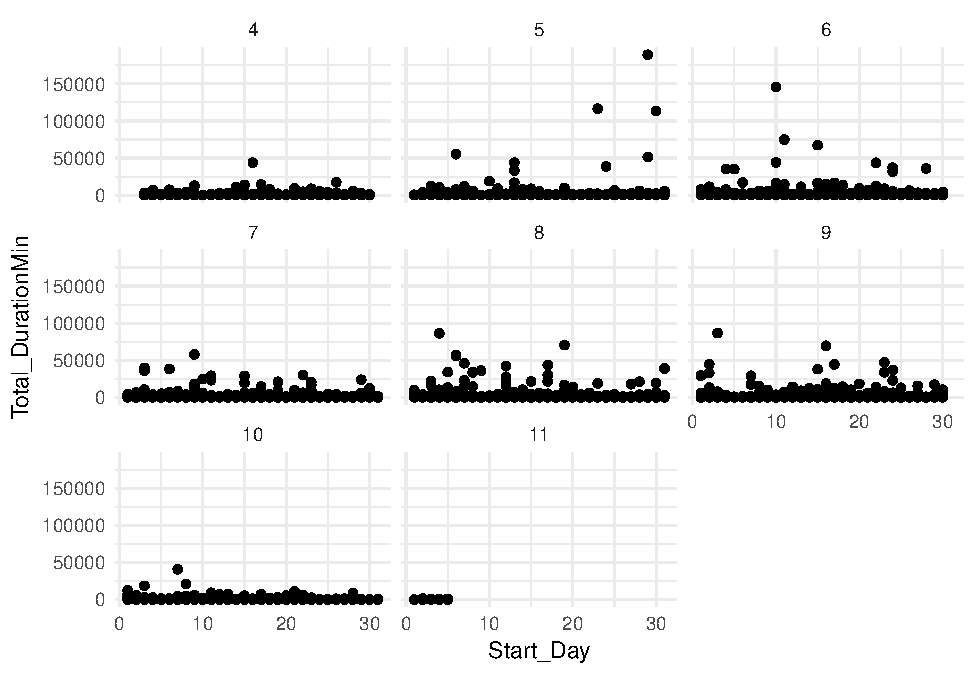
\includegraphics{Nice_Ride_Project_Stat_ReportDRAFT_files/figure-latex/unnamed-chunk-16-1.pdf}

\subsection{Geospatial exploration - busiest starting stations in
Minneapolis}\label{geospatial-exploration---busiest-starting-stations-in-minneapolis}

\begin{Shaded}
\begin{Highlighting}[]
\CommentTok{#Load map}
\NormalTok{Map_TwinCities <-}\StringTok{ }\KeywordTok{get_map}\NormalTok{(}\KeywordTok{c}\NormalTok{(}\DataTypeTok{lon =} \OperatorTok{-}\FloatTok{93.25576}\NormalTok{, }\DataTypeTok{lat =} \FloatTok{44.97394}\NormalTok{), }\DataTypeTok{zoom =} \DecValTok{12}\NormalTok{, }\DataTypeTok{maptype =} \StringTok{"roadmap"}\NormalTok{, }\DataTypeTok{source =} \StringTok{"google"}\NormalTok{)}
\end{Highlighting}
\end{Shaded}

\begin{verbatim}
## Map from URL : http://maps.googleapis.com/maps/api/staticmap?center=44.97394,-93.25576&zoom=12&size=640x640&scale=2&maptype=roadmap&language=en-EN&sensor=false
\end{verbatim}

\begin{Shaded}
\begin{Highlighting}[]
\CommentTok{#Set map data subset of Rides}
\NormalTok{Geo_Rides <-}\StringTok{ }\NormalTok{Rides }\OperatorTok\StringTok{ }\KeywordTok{group_by}\NormalTok{(Start_Longitude, Start_Latitude) }\OperatorTok\StringTok{ }\KeywordTok{count}\NormalTok{(Start_Station) }\OperatorTok\StringTok{ }\KeywordTok{arrange}\NormalTok{(}\KeywordTok{desc}\NormalTok{(n))}

\KeywordTok{attach}\NormalTok{(Geo_Rides)}
\end{Highlighting}
\end{Shaded}

\subsubsection{Observe bike stations by number of trips for the
season}\label{observe-bike-stations-by-number-of-trips-for-the-season}

\begin{Shaded}
\begin{Highlighting}[]
\KeywordTok{ggmap}\NormalTok{(Map_TwinCities) }\OperatorTok{+}\StringTok{ }\KeywordTok{geom_point}\NormalTok{(}\KeywordTok{aes}\NormalTok{(}\DataTypeTok{x =}\NormalTok{ Start_Longitude, }\DataTypeTok{y =}\NormalTok{ Start_Latitude, }\DataTypeTok{size =}\NormalTok{ n), }\DataTypeTok{data =}\NormalTok{ Geo_Rides, }\DataTypeTok{alpha =}\NormalTok{ .}\DecValTok{25}\NormalTok{, }\DataTypeTok{color =} \StringTok{"blue"}\NormalTok{)}
\end{Highlighting}
\end{Shaded}

\begin{verbatim}
## Warning: Removed 34 rows containing missing values (geom_point).
\end{verbatim}

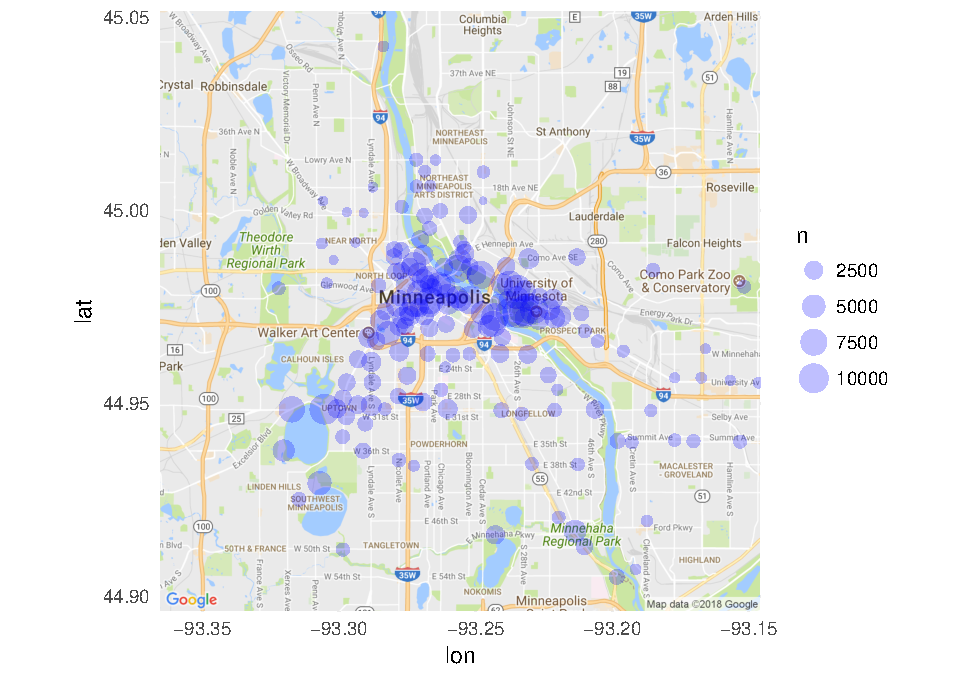
\includegraphics{Nice_Ride_Project_Stat_ReportDRAFT_files/figure-latex/unnamed-chunk-18-1.pdf}

The stations with the highest volume are in the downtown metro,
University of Minnesota west bank campus and the lake of the Calhoun
Isles area. \emph{Mapping the station volume brought 34 rows containing
missing values to our attention.}

\subsection{Next steps, changes in research purpose and intended
outcome}\label{next-steps-changes-in-research-purpose-and-intended-outcome}

Next steps are:

\begin{itemize}
\item
  Address outliers and dataset concerns brought forth in the EDA process
  before moving on to next phase
\item
  Evaluate intended application of the project. The goal of this project
  remains focused on exploring how weather impacts bike share volume,
  but we must also consider other variables. \emph{Should we account for
  holidays as they alter weekday ridership into patterns more closely
  tied to weekend use? What other variables affect ridership besides
  weather? City events?}
\item
  The ultimate goal is to build a predictive model that shows how an
  altering of weather variables affects ride volume for a given day.
  \emph{We have not explored the impact of ridership from our weather
  type categorical variable.}
\end{itemize}


\end{document}
